\newpage
\section{Design Considerations}

\subsection*{Architecture}

Figure~\ref{fig:architecture-diagram} shows the architecture of this application:

\begin{figure}[ht]
  \centering
  \includegraphics*[width=\textwidth]{assets/images/diagrams/architecture-diagram.png}
  \caption{Architecture of the application}
  \label{fig:architecture-diagram}
\end{figure}

\subsection*{Type of Blockchain}

To satisfy \textbf{NF\_M1} and \textbf{NF\_M2}, we will need to use a public blockchain, which will benefit our project by:

\begin{itemize}
  \item being accessible to a larger user-base, which should boost availability and scalability (\textbf{NF\_S1}),
  \item reducing the risk of censorship (\textbf{NF\_M1}), and
  \item providing greater data integrity (\textbf{NF\_M4})
\end{itemize}

\noindent Ethereum is a public blockchain that allows developers to publish their own distributed applications to it. It comes with an extensive development toolchain so is an obvious choice for this project (\textbf{F\_M8}).

\subsection*{Uploading Content}
\label{subsec:upload-content}

For developers to upload their game (\textbf{F\_M5}), they must provide a digital certificate to prove their identity (\textbf{NF\_M3}) as well as the required metadata (\textbf{F\_M1}) for identifying\footnote{Such as the name, release date, version number, creator and price.},
downloading\footnote{Such as the address of where to purchase the game, the digital certificate of who you're purchasing off and a tracker} and verifying their game\footnote{The root hash and the hashes of each block of data}. 
The developer is then expected to allow users to purchase the game off them and seed the game to at least an initial group of users.

\begin{figure}[ht]
  \centering
  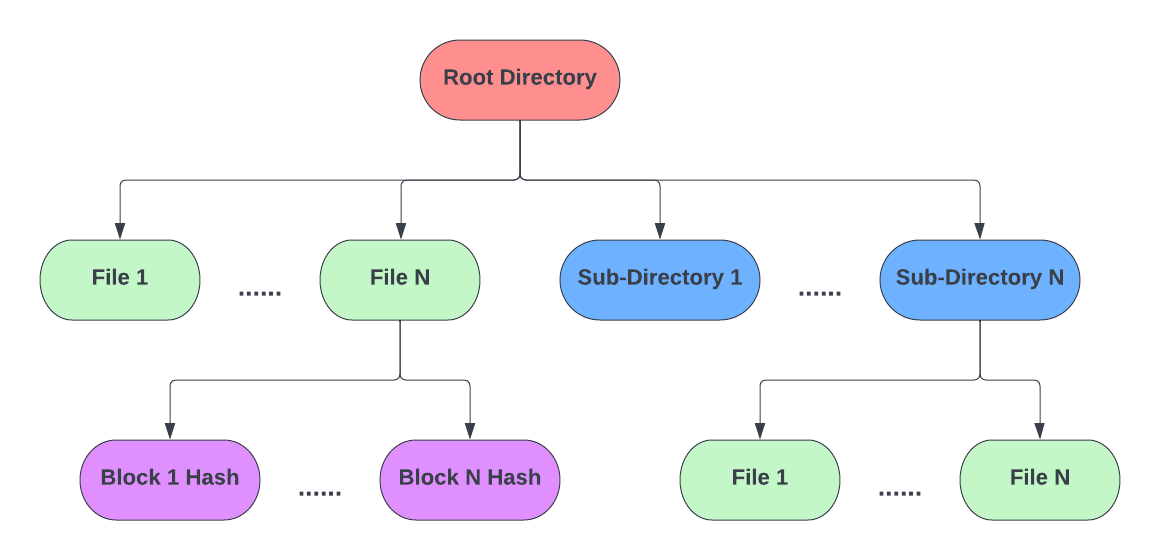
\includegraphics[width=.85\textwidth]{assets/images/diagrams/block-body.png}
  \caption{Hash data about shards will be stored in a tree that mimics the folder structure of the data}
  \label{fig:hash-storage}
\end{figure}

\subsection*{Purchasing Content}

Users will purchase content from developers using Ether (\textbf{F\_M9}) and will be provided with a proof of purchase (\textbf{F\_M10}) that is encrypted with the developer's private key. By using public key infrastructure, it gives proof of purchases authenticity that allows them to be validated by any node in the network. 
The proof of purchase will include: the root hash of the title purchased, the developer's address, the purchaser's address, a timestamp, and a unique seeder token to be used for proving distribution.

\subsection*{Downloading Content}

Games will be content addressable, using their root hash stored on the blockchain. This will allow nodes to connect with each other based on the content they are interested in (\textbf{F\_M3}). Once a user connects to a node it will:

\begin{enumerate}
  \item Send their proof of purchase (\textbf{F\_S2}).
  \item request individual shards from the node using the shard's hash (\textbf{F\_M2}),
  \item use the metadata from the blockchain to verify the shard's contents (\textbf{F\_M7}),
  \item send a confirmation message that proves the successful transfer of a block (\textbf{F\_S1}), 
  \item and repeat this until the entirety of the game is installed (\textbf{F\_M6}).
\end{enumerate}

\noindent As the blockchain will only be used to store metadata about games uploaded to the network, not every node will have each game installed. Instead, this project will take ideas from networks like BitTorrent, where nodes will seek out peers who have the game installed using a tracker hosted by the uploader.

\subsection*{Updating Content}

To satisfy \textbf{F\_M4}, developers will perform the same steps as in \textbf{Uploading Content} but will also include the hash of a previous block that contains the older version of the game. This will include the restriction that only the original uploader can upload an update for their game (\textbf{NF\_S2}).

\begin{figure}[ht]
  \centering
  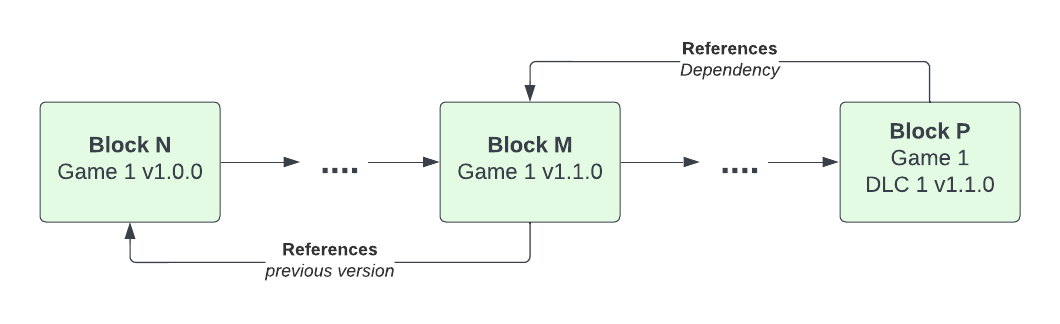
\includegraphics[width=.85\textwidth]{assets/images/diagrams/software.png}
  \caption{How blocks relate to each other. An update will reference the previous version whilst a DLC will reference, which piece of software and version it is dependent on.}
\end{figure}

\noindent It is likely that many shards will persist between versions so a node will only ever download the changed or new data. To satisfy \textbf{F\_C1}, a node may optionally keep older shards that have been removed or changed.

\subsection*{Downloadable Content}

Developers will typically offer paid or free DLC (\textbf{F\_S3}) for their games that users will purchase separately. Each DLC will need:

\begin{enumerate}
  \item \textbf{Dependency} A reference to the oldest version of the game they apply to, and
  \item \textbf{Previous Version} A pointer to the previous
\end{enumerate}

\subsection*{Proving Contribution}

When a user purchases a piece of software they will be granted a unique seeder token. When a user successfully downloads a shard of data off of a peer they will reply with a confirmation message, containing their seeder token, that is encrypted using the developers public key. 
When a user wants to prove that they have contributed to the distribution of a game, they will send a collection of these messages to the developer, who will judge their validity.

\subsection*{Sequence Diagram}

Figure~\ref{fig:sequence-diagram}, shows the main interactions for a game uploaded to the network and how different actors will interact with each other.

\begin{figure}[ht]
  \centering
  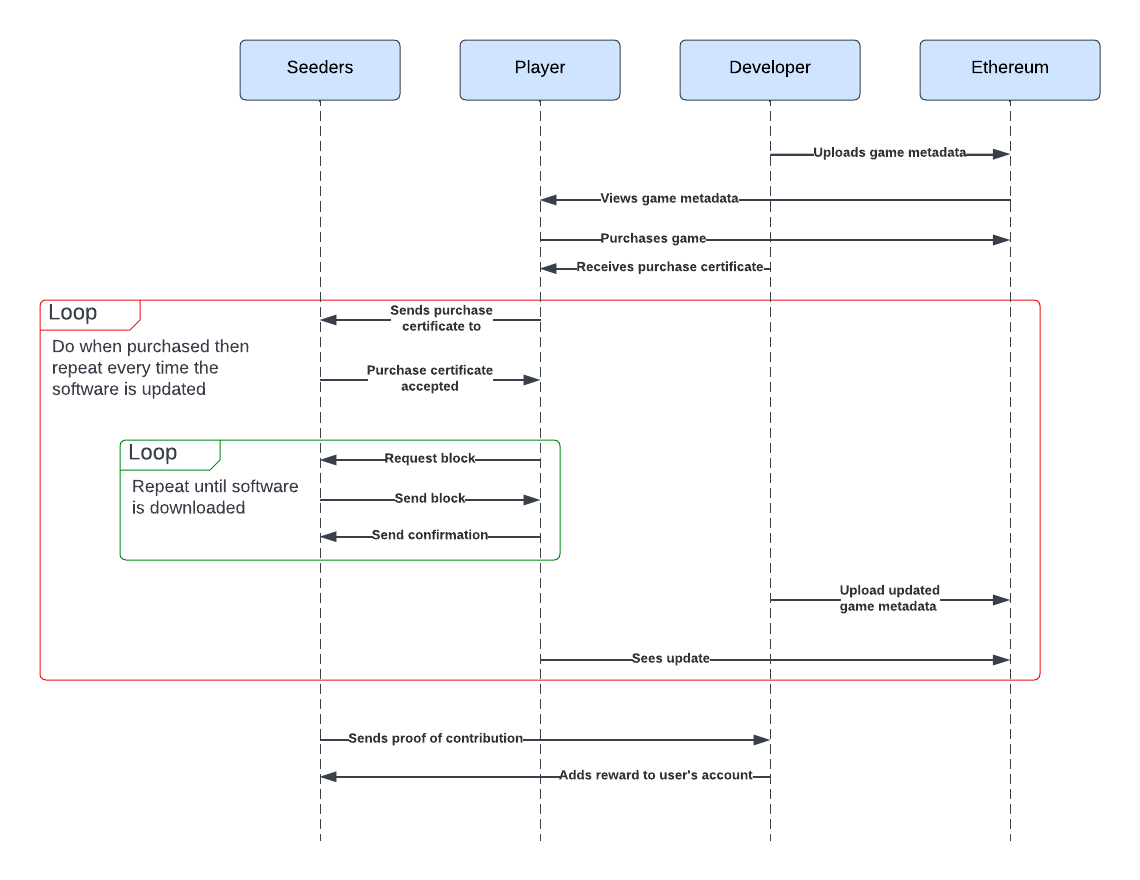
\includegraphics[width=.95\textwidth]{assets/images/diagrams/seqeunce-diagram.png}
  \caption{A sequence diagram showing some of the main interactions within this application}
  \label{fig:sequence-diagram}
\end{figure}